\documentclass[a4paper, 12pt]{article}
\usepackage{graphicx}
\usepackage{amsmath}
\usepackage{amsthm}
\usepackage{amssymb}
\usepackage{url}
\usepackage{multirow}
\usepackage{times}
\usepackage{fullpage}
\usepackage{float}
\usepackage{hyperref}
\usepackage[usenames,dvipsnames]{xcolor}
\newcommand{\comment}[1]{}

\hypersetup{
  colorlinks   = true,    % Colours links instead of ugly boxes
  urlcolor     = black,    % Colour for external hyperlinks
  linkcolor    = SkyBlue,    % Colour of internal links
  citecolor    =SkyBlue      % Colour of citations
}

\begin{document}

\begin{titlepage}
\center

\includegraphics[scale=0.8]{logo.png}\\[1cm]
{\huge \bfseries IITK Academic Calender}\\[0.4cm]
\center
{\huge Project Report }
\center
\begin{tabular}{ccc}
	SUDHIR  & AMAN KUMAR & RAHUL P\\
	12734 & 12085 & 12539 \\
	\href{mailto:sudkumar@iitk.ac.in}{\nolinkurl{sudkumar}} &\href{mailto:amanku@iitk.ac.in}{\nolinkurl{amanku}} & \href{mailto:rahulpv@iitk.ac.in}{\nolinkurl{rahulpv}}\\ 
	\multicolumn{3}{c}{}\\
	\multicolumn{3}{c}{\large Group 25}
\end{tabular}
\center
\large \today\\[2cm]
\end{titlepage}
\newpage
\tableofcontents

\newpage
\begin{abstract}
An academic calendar for IITK community to see all their registered academic events.
\end{abstract}

\section{Introduction}
This academic calendar is for students and professors to keep track of all the ongoing academic events in the campus.Updates are made regularly
in the calendar for the events like quizzes, extra classes, labs and etc.
\subsection{Project Overview}
For professors:-
\begin{itemize}
  \item Professors are sent OTP(One Time Password)or can register(only for testing purpose) to activate their account.
  \item After sign-in for the first time they are redirected to a page where they are to fill a form inputting the course details and upload a .txt file with roll numbers of the students enrolled in that particular course.
  \item In-case a professor is teaching multiple courses in a single semester, options are provided at the top left of the page to select the course of their choice.
  \item Once the course is selected a calendar is displayed which showcases the merged events of all the students enrolled in that course.
  \item Selecting a particular date will display the events scheduled on that day.The events planned by singed-in user can be modified or deleted by the user himself and no one else.
\end{itemize}
For students:-
\begin{itemize}
  \item Students are sent OTP(One Time Password) or can register(only for testing purpose) to activate their account.
  \item After sign-in, a particular student is shown his/her calendar and the events of the courses they are registered in.
  \item Selecting a particular date on the calendar will display all the academic activities scheduled on that day for that student.
  \item A notification is shown on the top of the page if there is new event added in the student's calendar.
\end{itemize}

\section{Methodology}
\subsection{Front end}
Various parts of the front end are made using the mixture of HTML, CSS, and Java Script.Server side scripting is done using PHP and MySql.To make it a single page application AngularJS javascript framework is used.For web designing, bootstrap twitter has been used.
\subsection{Back end}
Everything is maintained in a single SQL database consisting of 6 tables.Different types of actions such as Add event, Edit event, Delete event, merging events, adding of entries and etc. are done using PHP and their corresponding MySql quires.
\section{Overview of code}
The entire code is available at          \texttt{\href{https://github.com/sudkumar/calendar}{https://github.com/sudkumar/calendar}}. A little explanation on the code directory wise:-
\begin{description}
\item[cal.sql-] \hfill \\
This file contains the structure for database. If any one wants to use this code, they have to import this file in there database to make the structure for the project.

\item[core-] \hfill \\
This Folder contains two folders database, functions and a file init.php. init.php file combines all the files from these two folders and also initializes everything for the users. All the files are self explanatory with there name like database/connect.php, funtions/users.php. If any one wants to use this code, they have to change there hostname, username and password for connection to database server. This can be changed in database/connect.php.

\item[css-] \hfill \\
This contains all the css files used in different pages of this calendar.

\item[data-] \hfill \\
This folder contains all the PHP scripts that we have used for ajax calls from AngularJS. Files are seperated in two folders named fac(teachers) and std(students) to make better understanding. 

\item[fac-] \hfill \\
This is the teacher user interface part of our project. File index.php is the home for faculty and update.php and deleteCourse.php are self explanatory.

\item[fonts-] \hfill \\
This file contains all the font and icon files.

\item[js-] \hfill \\
All the interactions written in java script are stored here in this folder. Some files like angular-min, bootstrap-min, jQuery are taken from open sources and two files named facapp.js and stdapp.js are used for teachers and students user interaction respectively.

\item[std-] \hfill \\
This is the student user interface part of our project.


\item[index.php-] \hfill \\
This is the main file containing the code for login and registration for all the different scenarios.


\item[403.php and 404.php-] \hfill \\
These are for 403 and 404 http errors.

\end{description}

\newpage
\section{Results}

The present GUI of the calendar for the student home.

\begin{figure}[H]
	\caption{GUI of the calendar showing the events for the selected day for students}
	\vspace{.5cm}
	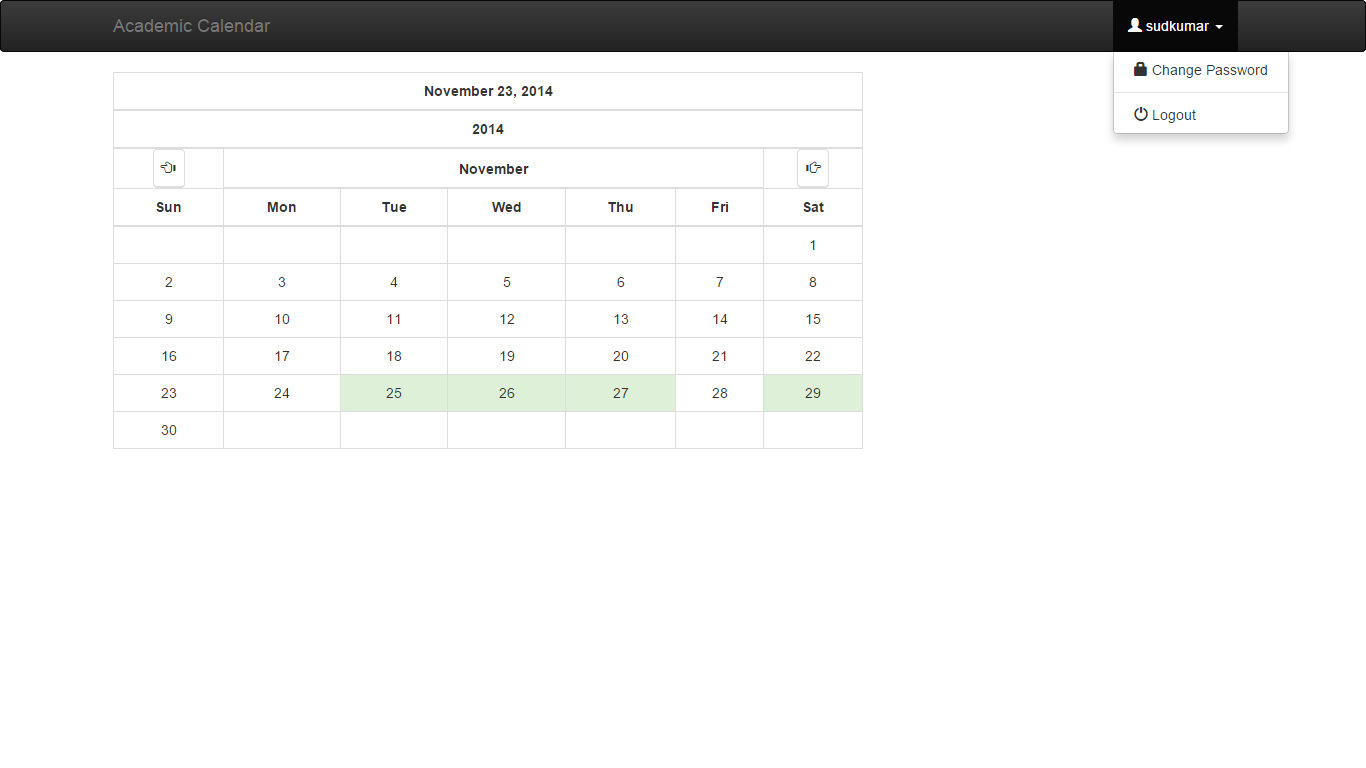
\includegraphics[width=0.95\columnwidth]{student_home2}
	\label{fig:figure1}
\end{figure}


\begin{figure}[H]
	\caption{GUI of the calendar for the Professor adding an event}
	\vspace{.5cm}
	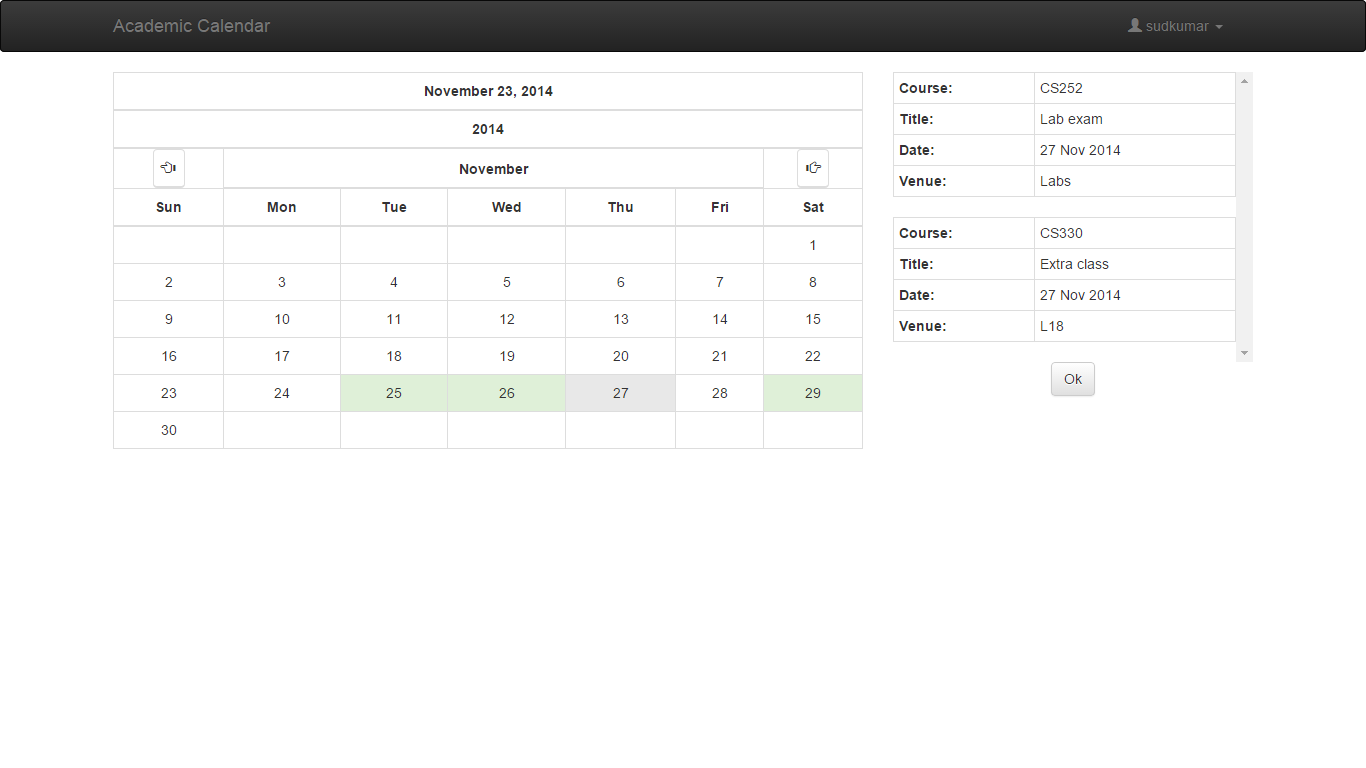
\includegraphics[width=0.95\columnwidth]{student_event}
	\label{fig:figure2}
\end{figure}

 
\begin{figure}[H]
	\caption{GUI for teachers to add event on selected date and course}
	\vspace{.5cm}
	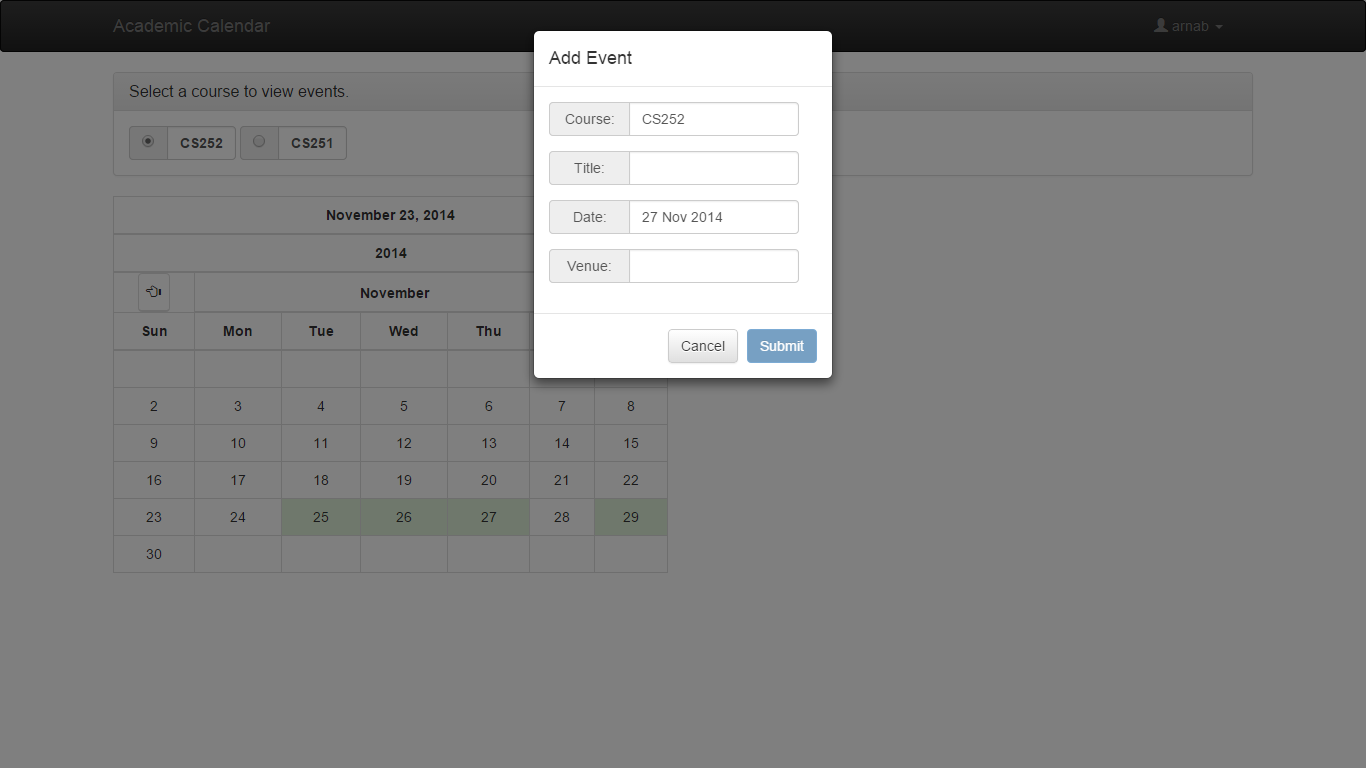
\includegraphics[width=0.95\columnwidth]{teacher_add_event}
	\label{fig:figure3}
\end{figure}
 
\begin{figure}[H]
	\caption{GUI for events to the teaches}
	\vspace{.5cm}
	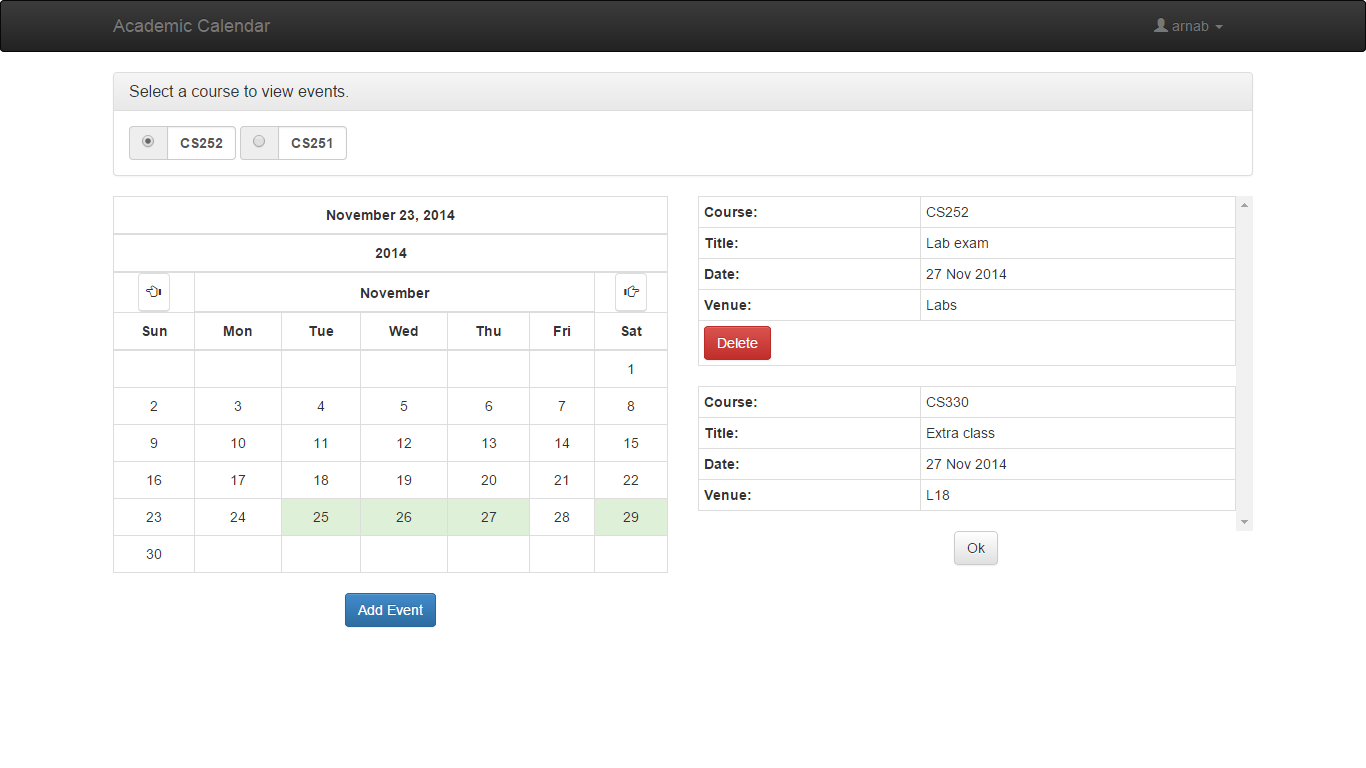
\includegraphics[width=0.95\columnwidth]{teacher_show_event}
	\label{fig:figure4}
\end{figure}

\begin{figure}[H]
	\caption{GUI for course updating for teachers}
	\vspace{.5cm}
	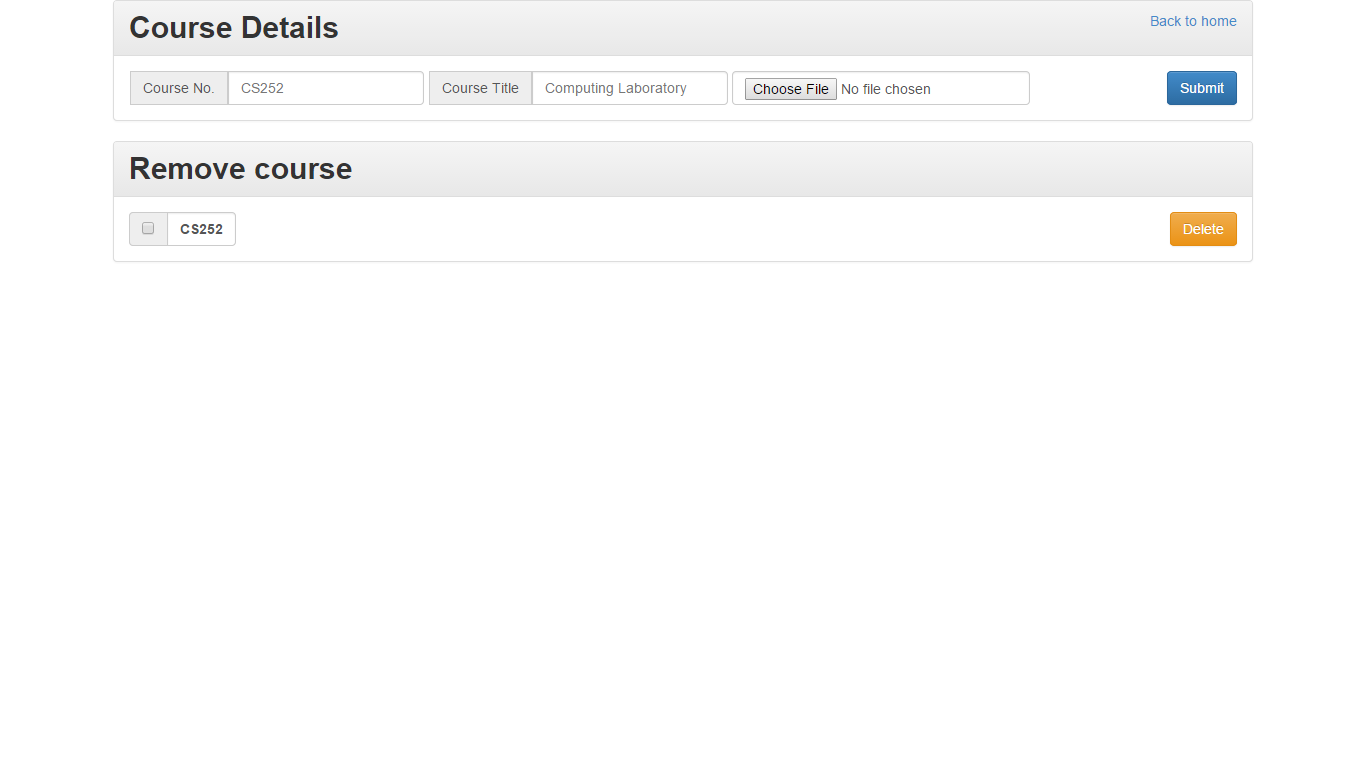
\includegraphics[width=0.95\columnwidth]{update_course}
	\label{fig:figure5}
\end{figure}

\section{Evaluation}
The product has been tested for known possible errors and fixes were given accordingly.In terms of security the database is encrypted and necessary measures are taken to prevent any possible tricks that can be done by URL manipulation. Source code isn't compatible with internet explorer and works perfect for google chrome and firefox.
\section{Tools}
The tools used were \texttt{\href{http://www.sublimetext.com/}{Sublime}} text editor for editing purpose and  \texttt{\href{https://www.apachefriends.org/index.html}{XAMPP}} for easy handling with server.
\section{Conclusions and Future Work}
In conclusion the project took about two and half weeks of work.It's present features are given in the introduction.The desired functionalities were met. And the code is well organized and is reusable.
For future work when this calendar is to be up and running for the IITK community all the details will be taken from the OARS server.Details such as CC login id and password and also the courses details which provide inputs such as the professor of the course and the students enrolled in the course.This makes the hefty job of the professor needing to upload the text file of roll no. of all the students enrolled in his courses.Further work can also be done on this calendar making it more personal and social by allowing students to follow(or add) the calendars of Snt Council,Cultural council,FMC council or any individual club.Id's are provides for the Secretaries and coordinators of councils and clubs respectively to add events in their calendars which will update the calendars of students following that particular council or club.

\end{document}
